\documentclass[11pt]{article}

% ---------- Packages (same preamble as Week 1) ----------
\usepackage[letterpaper,margin=1in]{geometry}
\usepackage[T1]{fontenc}
\usepackage{newtxtext,newtxmath}
\usepackage{microtype}
\usepackage{amsmath}  % newtxmath already provides the AMS symbols
\usepackage{booktabs,tabularx,array}
\usepackage{graphicx}
\usepackage[font=small,labelfont=bf]{caption}
\usepackage{float}
\usepackage{enumitem}
\usepackage{xcolor}
\usepackage{listings}
\usepackage[hidelinks]{hyperref}

\definecolor{codebg}{HTML}{F4F3EF}
\lstset{basicstyle=\ttfamily\footnotesize, backgroundcolor=\color{codebg},
        frame=none, xleftmargin=6pt, xrightmargin=6pt, aboveskip=6pt, belowskip=6pt,
        columns=fullflexible, keepspaces=true, breaklines=true}
\setlist{itemsep=2pt, topsep=4pt}
\graphicspath{{figures/}}
\newcolumntype{L}{>{\raggedright\arraybackslash}X}
\newcommand{\code}[1]{\texttt{#1}}
% Auto-generated by src/pipeline/run.py. Do not edit by hand.
\newcommand{\wRows}{1,761}
\newcommand{\wFeatures}{22}
\newcommand{\wChecks}{10}
\newcommand{\wGapdaysdgsone}{13}
\newcommand{\wGapdaysdff}{0}
\newcommand{\wGapmaxdiffpp}{0.165}
\newcommand{\wGaptotal}{78}
\newcommand{\wIqrlower}{-0.0333}
\newcommand{\wIqrupper}{0.0345}
\newcommand{\wFlagsonefive}{93}
\newcommand{\wFlagsthree}{21}
\newcommand{\wFlagsthreecovid}{13}
\newcommand{\wFlagsthreeoppvix}{18}
\newcommand{\wReversals}{2}
\newcommand{\wGdeltmissing}{4}
\newcommand{\wAnchorrv}{27.2}
\newcommand{\wAnchorq}{2.30}
\newcommand{\wAnchorr}{0.06}
\newcommand{\wSentnewsmean}{0.56}
\newcommand{\wSentconsmean}{0.39}
\newcommand{\wDatasethash}{0b8fef7a964a64ab}
\newcommand{\wMaxcorr}{0.996}
\newcommand{\wMaxcorrpair}{\texttt{r\_3m} and \texttt{r\_6m}}
\newcommand{\wFlagsonefiveshare}{5.3}
\newcommand{\wWeeklymatched}{365}
\newcommand{\wReversalsconfirmed}{2}
\newcommand{\wGapmeandiffdgsone}{0.014}
\newcommand{\wGapmaxdiffdgsone}{0.045}
\newcommand{\wGdeltdays}{2,918}
\newcommand{\wGdeltarticlesmedian}{321}
\newcommand{\wTonetwentyfour}{+0.91}
\newcommand{\wToneprevmax}{+0.05}
\newcommand{\wAnchorrsameday}{0.07}
\newcommand{\wWarmuprows}{631}


% ---------- Title ----------
\title{\textbf{Cleaning the Data and Engineering Point-in-Time Features for JPM Chooser Option Pricing}\\[4pt]
\large Week 2 Lab Report: Data Preprocessing and Feature Engineering}
\author{Aiden Leong\\[2pt]
\small Goldman Sachs Online Internship, Quantitative Research \& Trading\\
\small Supervisor: Tyler Chan\\
\small \url{https://github.com/aiden-zl/advanced-chooser-option-pricing-model}}
\date{25 November 2026}

\begin{document}
\maketitle

\begin{abstract}
\noindent
I turn the Week~1 raw data into a cleaned, model-ready dataset of \wRows{} trading days and \wFeatures{} features,
built by an automated pipeline that runs every week on GitHub Actions. Every feature is point-in-time: on each day
it uses only information that was public by that day's close, and an automated test confirms this by rebuilding the
dataset with future data removed. Missing values are filled with the last published value rather than interpolated,
which avoids borrowing tomorrow's data at a cost of \wGapmeandiffdgsone{} percentage points on average. An IQR screen
flags \wFlagsthree{} extreme return days; three independent checks show they are genuine market moves, so all are
kept. Following the feasibility check promised in Week~1, the news-sentiment feature uses daily GDELT tone for
JPMorgan articles, and a second sentiment feature uses the University of Michigan consumer survey. The dataset
reproduces the Week~1 spot price, volatility and dividend yield exactly.
\end{abstract}

% =====================================================================
\section{Objective}
The project brief sets three tasks for Week~2:
\begin{enumerate}
  \item \textbf{Data cleaning:} handle missing values, outliers (IQR) and time alignment.
  \item \textbf{Feature engineering:} traditional features (rolling volatilities, daily returns, dividend growth) and
        advanced features (VIX--JPM correlation, interest-rate momentum, sentiment scores in $[0,1]$).
  \item \textbf{Pipeline development:} an automated preprocessing pipeline scheduled with GitHub Actions.
\end{enumerate}
Deliverables: a cleaned dataset (CSV/Parquet, at least 10 features), the pipeline code, and feature documentation
(delivered separately as \emph{Feature Engineering Documentation v1.0}).

% =====================================================================
\section{Background}
The machine-learning models in Weeks~5--6 will learn from these features. A common way such models look better in
testing than in real use is \emph{look-ahead bias}: a feature on some day accidentally contains information that was
not available yet, for example an inflation figure published three weeks later. I therefore treat every source as
point-in-time (Table~\ref{tab:pit}) and test for leaks directly.

\begin{table}[H]
\centering\small
\caption{When each source becomes usable on trading day $t$.}
\label{tab:pit}
\begin{tabularx}{\linewidth}{@{}>{\raggedright\arraybackslash}p{0.3\linewidth}>{\raggedright\arraybackslash}p{0.27\linewidth}L@{}}
\toprule
Source & Used on day $t$ & Reason \\
\midrule
JPM prices and dividends, VIX & Same day & Known at the close (VIX settles 15 minutes later). \\
Treasury yields, fed funds & Previous trading day & Published after the close or the next business day. \\
CPI, unemployment, consumer sentiment & First-published value, from its release date & Released weeks after the month and later revised. \\
GDELT news tone & Previous day & A GDELT day ends at midnight UTC, after the US close. \\
\bottomrule
\end{tabularx}
\end{table}

% =====================================================================
\section{Methods}
\subsection{Additional raw data}
Week~1's raw files are left untouched. Week~2 adds new raw files only (\code{src/pull\_week2.py}):
\begin{itemize}
  \item \textbf{Warm-up history} from 1 July 2015 for JPM, VIX and the FRED daily series (\wWarmuprows{} extra trading
        days), so that 252-day volatility and year-on-year growth have values from 2 January 2018.
  \item \textbf{First releases} of CPI, unemployment and consumer sentiment from ALFRED, the St.~Louis Fed's archive
        of past data vintages, with the date each number was first published.
  \item \textbf{GDELT news tone}: daily average tone and article counts for articles mentioning ``JPMorgan'',
        2017--2024 (\wGdeltdays{} days, median \wGdeltarticlesmedian{} articles per day).
  \item \textbf{Alpha Vantage weekly closes}, used as an independent check of Yahoo's prices.
\end{itemize}
Raw files are immutable once committed: the pull script only downloads files that do not exist yet, because Yahoo
revises its adjusted prices slightly from one download to the next.

\subsection{Cleaning}
\begin{enumerate}
  \item \textbf{Time alignment.} Every series is mapped to the NYSE trading calendar using the rules in
        Table~\ref{tab:pit}.
  \item \textbf{Missing values.} Gaps are filled with the last published value. I chose this over the brief's
        suggested interpolation because linear interpolation fills a gap with help from the \emph{next} day's value,
        which is information a trader would not yet have.
  \item \textbf{Outliers.} Daily log returns $r_t=\ln(S_t/S_{t-1})$ are flagged if they fall outside
        $[Q_1 - k\,\mathrm{IQR},\ Q_3 + k\,\mathrm{IQR}]$ for $k = 1.5$ and $k = 3$, where $Q_1$ and $Q_3$ are the
        lower and upper quartiles and $\mathrm{IQR}=Q_3-Q_1$. \emph{In words: a return is unusual if it is far outside
        the range of the middle half of all returns.} Flagged days are verified, not deleted.
  \item \textbf{Structural checks.} Duplicate dates, non-positive prices, closes outside the day's high--low range
        and zero-volume days.
\end{enumerate}

\subsection{Features}
Table~\ref{tab:featsum} summarizes the \wFeatures{} features; the feature documentation gives every formula. The
sentiment scores use an \emph{expanding percentile}: each day's value is ranked against all earlier values, so a score
of 0.9 means more positive than 90\% of everything seen so far, without using any future data.

\begin{table}[H]
\centering\small
\caption{Feature groups. Brief items are marked $\star$.}
\label{tab:featsum}
\begin{tabularx}{\linewidth}{@{}>{\raggedright\arraybackslash}p{0.2\linewidth}>{\raggedright\arraybackslash}p{0.38\linewidth}L@{}}
\toprule
Group & Features & Plain-English meaning \\
\midrule
Returns $\star$ & \code{ret\_1d} & Today's percentage move (log scale). \\
Rolling volatility $\star$ & \code{rv\_21}, \code{rv\_63}, \code{rv\_252}, \code{park\_21} & How much the price has been swinging over the last month, quarter or year; \code{park\_21} uses daily highs and lows. \\
Liquidity & \code{volume\_ratio\_21} & Today's trading volume relative to the last month. \\
Dividends $\star$ & \code{div\_ttm}, \code{div\_yield}, \code{div\_growth\_yoy} & Last year's dividends, the yield $q$ and its year-on-year growth. \\
VIX link $\star$ & \code{vix}, \code{corr\_jpm\_vix\_63} & Market fear level, and how closely JPM has moved with it. \\
Rates $\star$ & \code{r\_3m}, \code{r\_6m}, \code{r\_1y}, \code{slope\_10y\_3m}, \code{rate\_mom\_21}, \code{rate\_mom\_63}, \code{fed\_funds} & Risk-free rates, the yield-curve slope, and rate momentum (how much the 1-year rate rose or fell over 1 and 3 months). \\
Macro & \code{cpi\_yoy}, \code{unrate} & Inflation and unemployment as first published. \\
Sentiment $\star$ & \code{sent\_news}, \code{sent\_consumer} & JPMorgan news tone and US consumer mood, each scaled to $[0,1]$. \\
\bottomrule
\end{tabularx}
\end{table}

\subsection{Pipeline, scheduling and tests}
\code{python -m src.pipeline.run} builds the dataset from the committed raw files, runs \wChecks{} validation checks and
refuses to write output if any fail. It writes \code{data/processed/features\_daily.parquet}, an identical CSV, a feature
dictionary and a cleaning log. Because it needs no API keys, it runs on GitHub Actions without storing any secrets: the
workflow \code{.github/workflows/preprocessing.yml} runs every Monday, on every code change and on demand, executes the
checks and the test suite, and saves the dataset as a downloadable artifact. The offline test suite
(\code{python -m pytest}, 10 tests) covers:
\begin{itemize}
  \item \textbf{Look-ahead test.} The dataset is rebuilt with all data published after a cut-off date removed, at five
        cut-off dates; every value up to the cut-off must be unchanged. If a feature used future data, it would change.
  \item \textbf{Completeness and ranges}, the \textbf{Week~1 anchors}, \textbf{CSV equals Parquet}, the committed
        dataset equals a fresh rebuild, and two rebuilds are identical.
\end{itemize}

% =====================================================================
\section{Results}
\subsection{Additional raw data}
All 16 checks on the new raw files pass: the warm-up files join the Week~1 files without gaps, every month 2015--2024
has a first release published after its reference month, GDELT covers 99.9\% of days, and the Alpha Vantage weekly
closes match Yahoo in all \wWeeklymatched{} weeks.

\subsection{Missing values}
\begin{figure}[H]
\centering
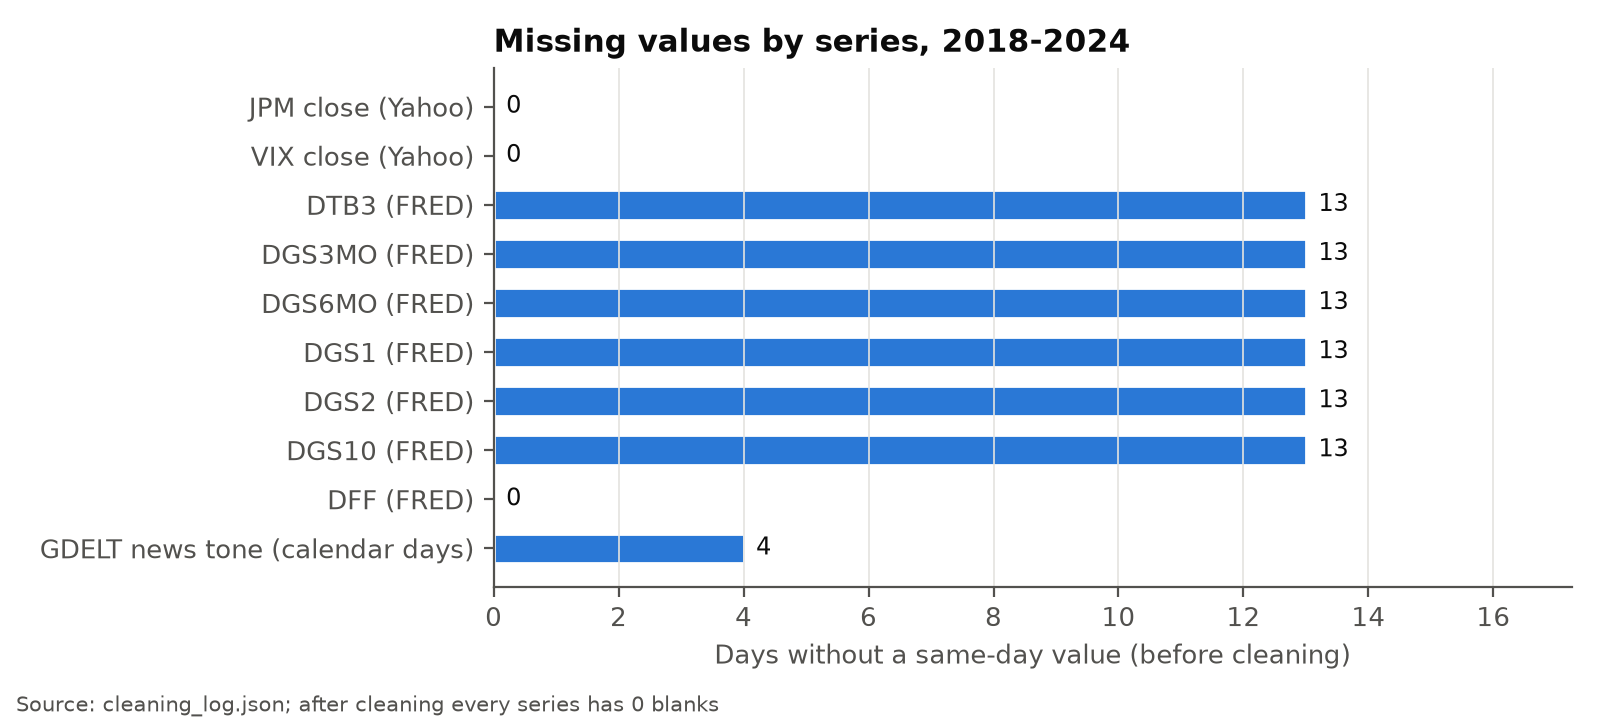
\includegraphics[width=0.92\linewidth]{fig1_missing_values.png}
\caption{Trading days in 2018--2024 with no same-day value, before cleaning. Data check: the only gaps are
\wGapdaysdgsone{} bond-market holidays in each Treasury series and \wGdeltmissing{} GDELT outage days; after cleaning
the dataset has no blanks.}
\label{fig:gaps}
\end{figure}
On the \wGapdaysdgsone{} gap days, previous-value fill and linear interpolation differ by \wGapmeandiffdgsone{}
percentage points on average for the 1-year yield (at most \wGapmaxdiffdgsone{}), so avoiding interpolation costs
almost nothing.

\subsection{Outliers}
\begin{figure}[H]
\centering
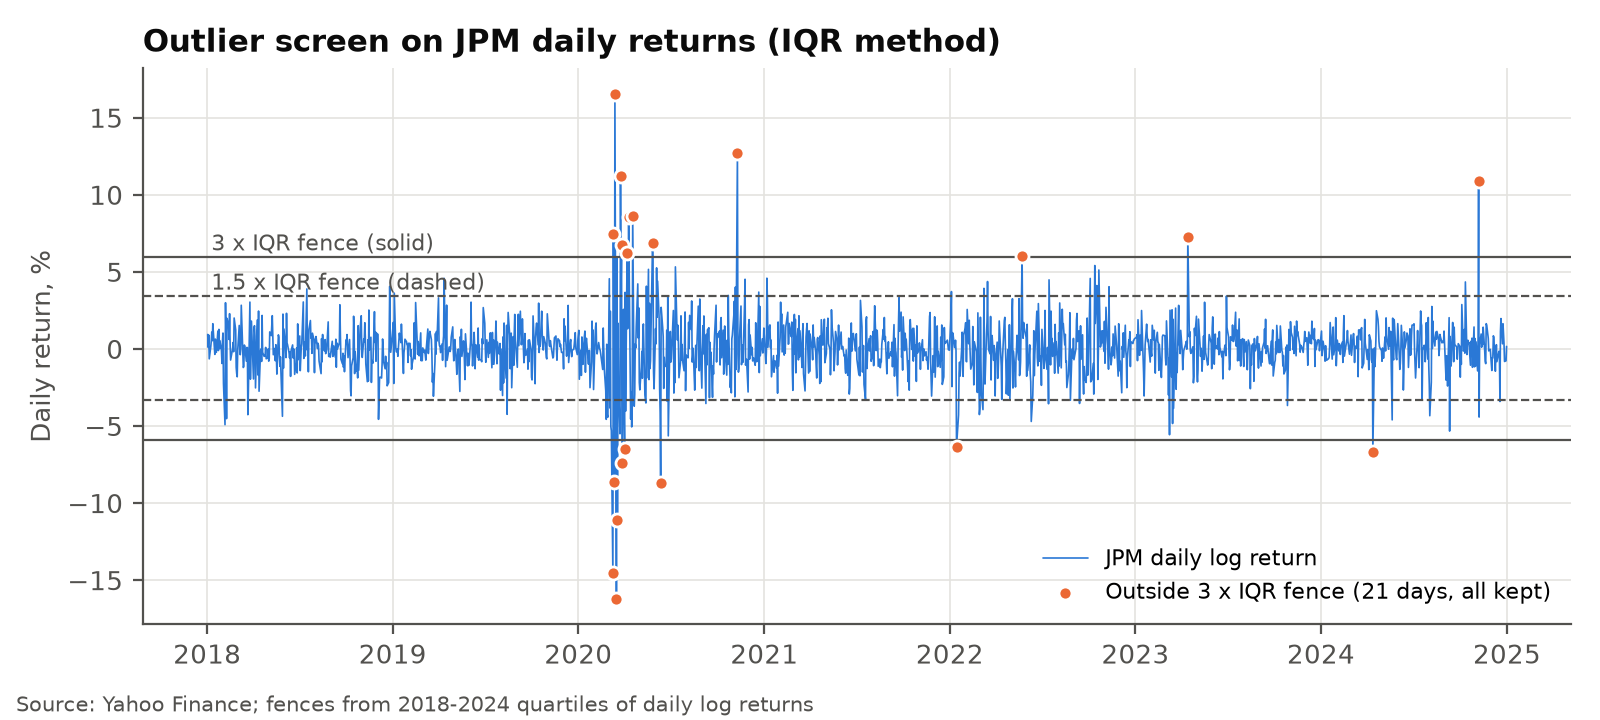
\includegraphics[width=\linewidth]{fig2_outliers.png}
\caption{IQR screen on JPM daily returns. Data check: \wFlagsonefive{} days lie outside the 1.5$\times$IQR fence and
\wFlagsthree{} outside the 3$\times$IQR fence, \wFlagsthreecovid{} of them during the COVID-19 crash. All are kept.}
\label{fig:outliers}
\end{figure}
Three checks show the flagged returns are real rather than data errors. (i) Alpha Vantage's weekly closes match Yahoo in
all \wWeeklymatched{} weeks. (ii) On \wFlagsthreeoppvix{} of the \wFlagsthree{} extreme days the VIX moved the opposite
way to JPM, as it does in genuine market stress. (iii) Only \wReversals{} days look like a one-day spike that reverses
the next day, the usual sign of a bad price; both (13 and 26 March 2020) are confirmed by the VIX and by the weekly
closes. Removing these days would hide the high-volatility periods the project is about.

\subsection{The feature dataset}
\begin{figure}[H]
\centering
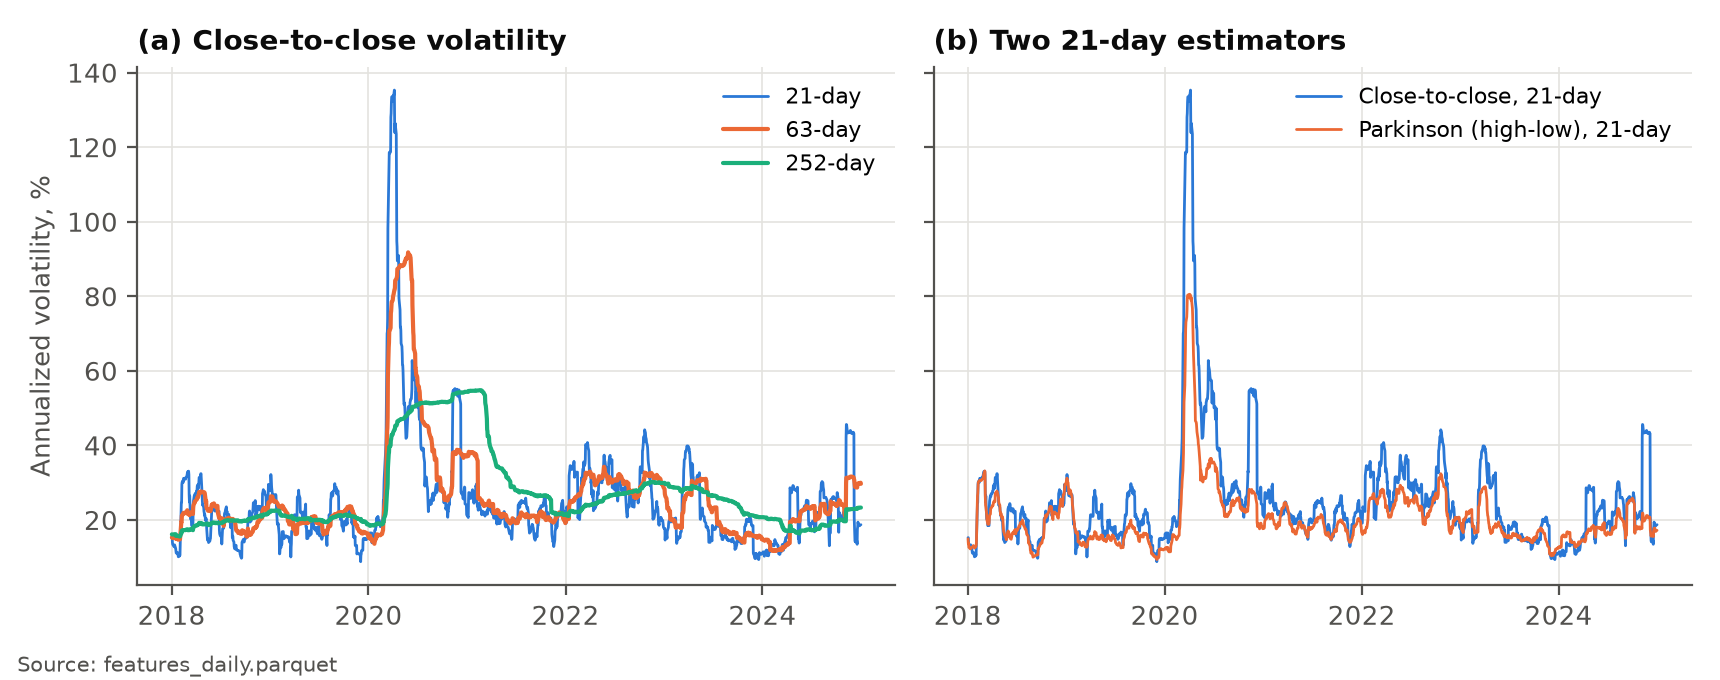
\includegraphics[width=\linewidth]{fig3_volatility_features.png}
\caption{Volatility features. Data check: all four are positive on every day, longer windows are smoother, and the
high--low estimator tracks the close-to-close one.}
\label{fig:vol}
\end{figure}

\begin{figure}[H]
\centering
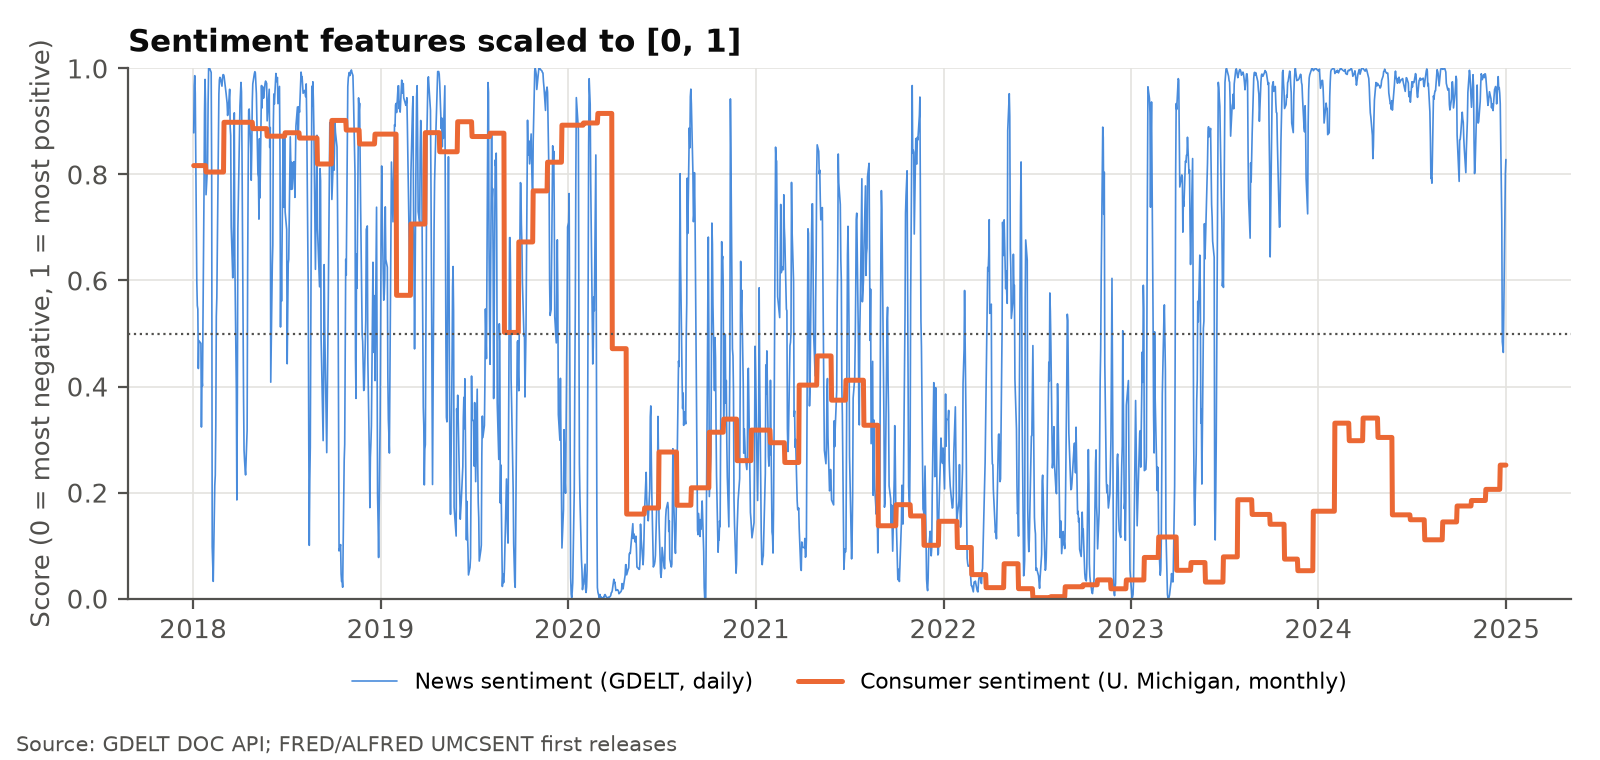
\includegraphics[width=\linewidth]{fig4_sentiment.png}
\caption{Sentiment features. Data check: both stay within $[0,1]$ on every day; news sentiment changes daily and
consumer sentiment steps once a month on its release date.}
\label{fig:sent}
\end{figure}

\begin{figure}[H]
\centering
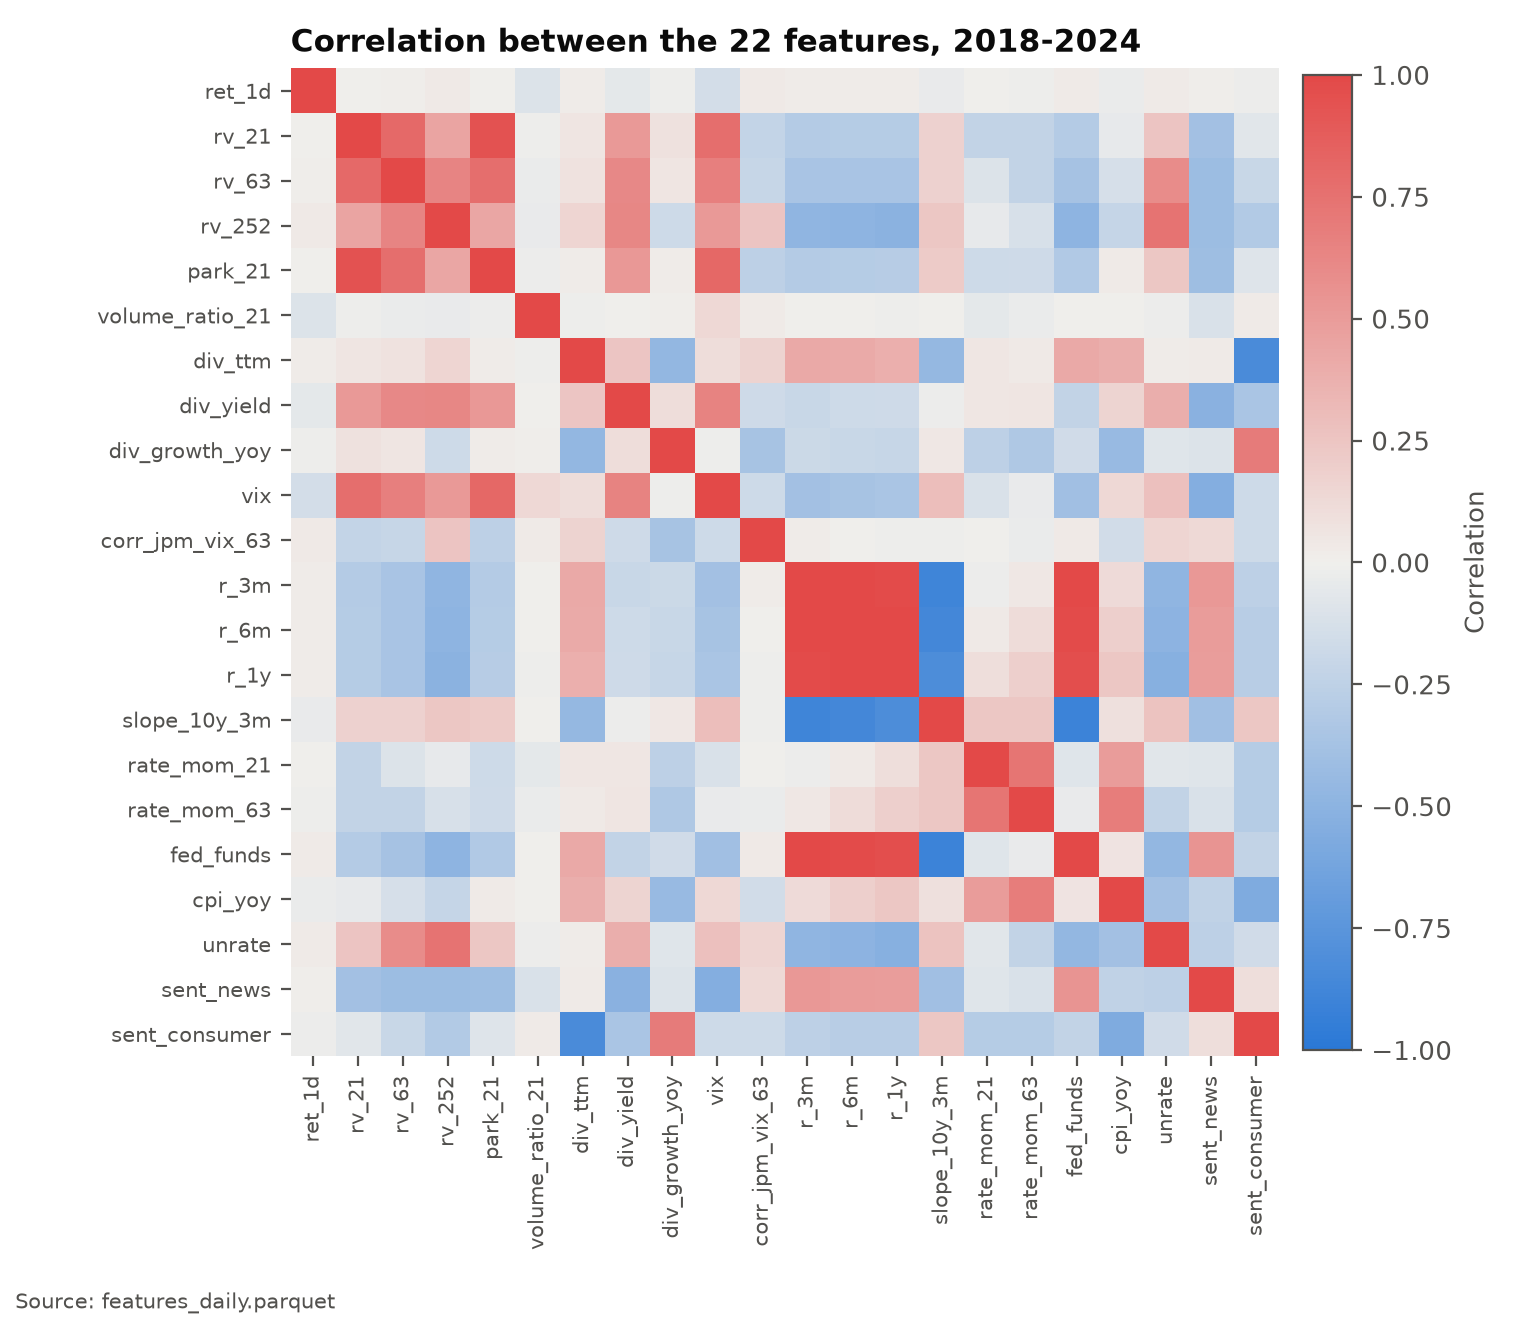
\includegraphics[width=0.82\linewidth]{fig5_feature_correlation.png}
\caption{Correlation between features. Data check: no two features are duplicates; the largest correlation is
\wMaxcorr{}, between \wMaxcorrpair{}.}
\label{fig:corr}
\end{figure}

\subsection{Validation, tests and the scheduled run}
All \wChecks{} pipeline checks and all 10 tests pass. On 23 August 2021 the dataset reproduces the Week~1 values exactly:
$S_0=\$156.70$, $\sigma=\wAnchorrv\%$ and $q=\wAnchorq\%$. The risk-free rate reads \wAnchorr\%: under the
point-in-time rule it is the previous trading day's 1-year yield, one basis point below the same-day \wAnchorrsameday\%
quoted in Week~1. The GitHub Actions workflow ran successfully on GitHub's servers in under a minute and published the
dataset as an artifact. Builds on macOS and on GitHub's Linux machines agree to within $10^{-13}$ (relative), the
expected difference between the two systems' math libraries.

% =====================================================================
\section{Discussion}
\paragraph{Deviations from the brief.} Two choices differ from the brief's wording, both to prevent look-ahead bias:
gaps are filled with the last published value instead of interpolated, and outliers are flagged and verified instead
of removed.

\paragraph{Sentiment source.} The Week~1 specification proposed GDELT for historical news sentiment and named survey
data as a fallback. The feasibility check passed: GDELT's DOC API returns daily JPMorgan tone back to January 2017, so I
use it for \code{sent\_news} and keep the consumer survey as the market-level \code{sent\_consumer}.

\paragraph{Limitations.} GDELT's average JPMorgan tone in 2024 (\wTonetwentyfour{}) was far above any earlier year (the
highest earlier yearly average was \wToneprevmax{}), so the expanding percentile stays near 1 for most of 2024. The short-term rates are almost
perfectly correlated with each other. Both are noted for the feature-selection step in Week~5.

% =====================================================================
\section{Conclusion and next steps}
All three Week~2 deliverables are complete: a cleaned dataset of \wRows{} days and \wFeatures{} point-in-time features
in CSV and Parquet, an automated pipeline scheduled on GitHub Actions, and the feature documentation. Week~3 will code
the BSM chooser option model from the paper, configure the paper's parameters ($K=\$150$, $T_2=1$ year), and compare
its outputs with the paper's reported results.

% =====================================================================
\appendix
\section{Reproducing these results}
\begin{lstlisting}
git clone https://github.com/aiden-zl/advanced-chooser-option-pricing-model
cd advanced-chooser-option-pricing-model
python3 -m venv .venv && source .venv/bin/activate
pip install -r requirements.txt
python -m src.pipeline.run       # build dataset, 10 checks (offline, no keys)
python -m pytest -q              # 10 tests incl. look-ahead test
python -m src.week2_figures      # figures for this report
tectonic -X compile deliverables/week2/lab_report.tex
\end{lstlisting}

\begin{thebibliography}{9}\small\raggedright
\bibitem{huang2021} Z.~Huang, X.~Wang and W.~Wan. Exploration of JPMorgan chooser option pricing.
  \emph{BCP Business \& Management}, 15:93--102, 2021.
\bibitem{parkinson} M.~Parkinson. The extreme value method for estimating the variance of the rate of return.
  \emph{Journal of Business}, 53(1):61--65, 1980.
\bibitem{gdelt} The GDELT Project. GDELT DOC 2.0 API, \url{https://api.gdeltproject.org}. Accessed 25 November 2026.
\end{thebibliography}

\end{document}
